\begin{frame}{Principal Component Analysis (PCA)}
	\begin{minipage}{0.59\textwidth}
		\begin{block}{PCA}
			The goal is to find the linear subspace $P_k$ that best fits the $d$-dimensional data $\{x_i\}_{i=1}^N$ in the LS sense, i.e., find an orthogonal family of $k$ vectors $\{u_l\}_{l=1}^k$ that maximizes
			\begin{equation*}
					\sum_{l=1}^k\sum_{i=1}^N |u_l^Tx_i|^2.
			\end{equation*}
		\end{block}
	\end{minipage}
	\begin{minipage}{0.4\textwidth}
	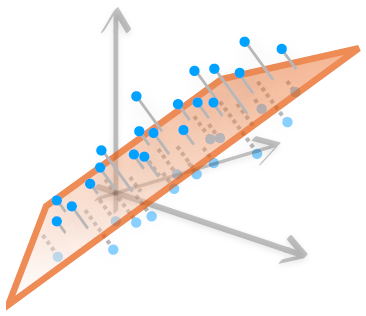
\includegraphics[width=\textwidth]{PCA_fig}
	\end{minipage}
	A solution is the $k$-principal eigenvectors of the empirical autocorrelation matrix
	\begin{equation*}
		\hat{R} = \frac{1}{N}\sum_{i=1}^N x_ix_i^T =: \frac{1}{N}\sum_{i=1}^N \Phi(x_i).
	\end{equation*}
	$\hat{R}$ is a \emph{sketch} of our data (of dim $d^2$).
\end{frame}


\begin{frame}
	The sketch 
	\begin{equation*}
		\hat{R} = \frac{1}{N}\sum_{i=1}^N x_ix_i^T =: \frac{1}{N}\sum_{i=1}^N \Phi(x_i) \in \mathbb{R}^{d^2}
	\end{equation*}
 	is a very compressed version of the data $\{x_i\}_{i=1}^N$, \emph{but}, it still contains the geometry of the data.
	\begin{block}{CS inspired idea}
		Take $m$ random measurements\footnote{$\mathcal{M}:\mathbb{R}^{d\times d}\to \mathbb{R}^m$ satisfying RIP on matrices of rank at most $2k$.} of each sample and use the sketch defined by $\Phi(x) = \mathcal{M}(xx^T)$. Provided $m>kd$, the principal eigenvectors can be recovered.
	\end{block}

\end{frame}